%%%%%%%%%%%%%%%%%%%%%%%%%%%%%%%%%%%%%%%%%%%%%%%%%%%%%%%%%%%%%%%%%%%%%%%%%%%%%%%%
\section{Snakefiles as Python-Code}
{   
	\usebackgroundtemplate{
		\vbox to \paperheight{\vfil\hbox to \paperwidth{\hfil\includegraphics[height=\paperheight]{logos/Text-x-python.svg.png}\hfil}\vfil}
		% source: https://en.m.wikipedia.org/wiki/File:Text-x-python.svg
	}
	\frame{
		\frametitle{Python Code in your Snakefile}
		\begin{mdframed}[tikzsetting={draw=white,fill=white,fill opacity=0.8,
				line width=0pt},backgroundcolor=none,leftmargin=0,
			rightmargin=150,innertopmargin=4pt,roundcorner=10pt]
			\tableofcontents[currentsection,sections={1-4},hideothersubsections]
		\end{mdframed}
	}
}

%%%%%%%%%%%%%%%%%%%%%%%%%%%%%%%%%%%%%%%%%%%%%%%%%%%%%%%%%%%%%%%%%%%%%%%%%%%%%%%%
\begin{frame}
  \frametitle{What is this about?}
   \begin{question}[Questions]
   	 \begin{itemize}
        \item How can I automatically manage dependencies and outputs?
        \item How can I use Python code to add features to my workflow?
        \item Will I be able to use my favourite script language, too?
     \end{itemize}
   \end{question}
   \begin{docs}[Objectives]
   	  \begin{enumerate}
         \item Use variables, functions, and imports in a Snakefile. 
         \item Learn to use the \altverb{run} action to execute Python code as an action and to \ldots
         \item \ldots use the \altverb{script} directive to execute arbitrary scripts (not just Python) conveniently using \Snakemake.
       \end{enumerate}
   \end{docs}
\end{frame}

%%%%%%%%%%%%%%%%%%%%%%%%%%%%%%%%%%%%%%%%%%%%%%%%%%%%%%%%%%%%%%%%%%%%%%%%%%%%%%%%
\subsection{Python Code in Snakefiles}

%%%%%%%%%%%%%%%%%%%%%%%%%%%%%%%%%%%%%%%%%%%%%%%%%%%%%%%%%%%%%%%%%%%%%%%%%%%%%%%%
\begin{frame}
  \frametitle{Why Python in a Snakefile?}
  Sometimes we do \emph{not} want to run $3^{\mathsf{rd}}$ party code, but run the occasional script for data manipulation   or plotting or \ldots 
  \pause
  \begin{docs}
  	\altverb{Snakefile}s are Python code (albeit special Python code)!)
  \end{docs}
\end{frame}

%%%%%%%%%%%%%%%%%%%%%%%%%%%%%%%%%%%%%%%%%%%%%%%%%%%%%%%%%%%%%%%%%%%%%%%%%%%%%%%%
\subsection{Supported Functions}

%%%%%%%%%%%%%%%%%%%%%%%%%%%%%%%%%%%%%%%%%%%%%%%%%%%%%%%%%%%%%%%%%%%%%%%%%%%%%%%%
\begin{frame}[fragile]
  \frametitle{Using functions in Snakefiles}
  We already met the \altverb{expand()}-function. Before we use Python in a \altverb{Snakefile}, let us discover some of \Snakemake's API together!
  \begin{task}
  	Start Python and follow along!
  \end{task}
  \begin{lstlisting}[language=Python,style=Python]
from snakemake.io import expand, glob_wildcards
  \end{lstlisting}
   \altverb{expand()} is used frequently, to expand a \Snakemake{} wildcard(s) into a set of filenames:
  \begin{lstlisting}[language=Python,style=Python]
>>> expand('folder/{wildcard1}_{wildcard2}.txt',
...        wildcard1=['a', 'b', 'c'],
...        wildcard2=[1, 2, 3])
  \end{lstlisting}
\end{frame}

% %%%%%%%%%%%%%%%%%%%%%%%%%%%%%%%%%%%%%%%%%%%%%%%%%%%%%%%%%%%%%%%%%%%%%%%%%%%%%%%%
\begin{frame}[fragile]
  \frametitle{Using functions in \altverb{Snakefile}s II}
  \begin{question}
  	What is the result?
  \end{question}
  \pause
  \begin{hint}[Answer:]
  	Every permutation of \altverb{wildcard1} and \altverb{wildcard2}!
  \end{hint}
  \pause
  Let us try \altverb{glob_wildcards()}, now:
  \begin{lstlisting}[language=Python,style=Python]
glob_wildcards('data/samples/{replicas}.fastq').replicas
  \end{lstlisting}
  \pause
  Wow! So, easy!
  \begin{question}
  	What happened? What happens if you leave \altverb{.replicas} away?
  \end{question}
\end{frame}

%%%%%%%%%%%%%%%%%%%%%%%%%%%%%%%%%%%%%%%%%%%%%%%%%%%%%%%%%%%%%%%%%%%%%%%%%%%%%%%%
\begin{frame}[fragile]
  \frametitle{\texttt{expand()} vs. \texttt{glob\_wildcards()}}
  \begin{exampleblock}{The Difference}
    \begin{columns}
      \begin{column}{0.45\textwidth}
        \begin{itemize}
         \item \altverb{expand()} is usefull to yield all permutations of wildcards
         \item \altverb{expand()} is oblivious to the underlying file system
        \end{itemize}

      \end{column}
      \begin{column}{0.45\textwidth}
        \begin{itemize}
         \item \altverb{glob_wildcards} infers files from wildcards
         \item \altverb{glob_wildcards} must be used with care - users tend to name files arbitrarily
        \end{itemize}

      \end{column}
    \end{columns}
  \end{exampleblock}
\end{frame}

%%%%%%%%%%%%%%%%%%%%%%%%%%%%%%%%%%%%%%%%%%%%%%%%%%%%%%%%%%%%%%%%%%%%%%%%%%%%%%%%
\subsection{Python Code as Actions}

%%%%%%%%%%%%%%%%%%%%%%%%%%%%%%%%%%%%%%%%%%%%%%%%%%%%%%%%%%%%%%%%%%%%%%%%%%%%%%%%
\begin{frame}[fragile]
  \frametitle{Meet the \texttt{run} Action}
  \vspace{-0.5em}
  It is possible to run Python snippets in \Snakemake{}. For this, we have to replace the \altverb{shell:} action by a \altverb{run:} action:\vspace{-0.5em}
  \begin{task}
  	Imagine this code in our \altverb{Snakefile}:
  \end{task}\vspace{-0.5em}
  \begin{lstlisting}[language=Python,style=Python, basicstyle=\footnotesize]
# will plot the positions of our detected deviations
# from the reference
rule plot_positions:
    run:
        import matplotlib
        ...
  \end{lstlisting}
  \vspace{-0.5em}
  \pause\footnotesize
  \begin{hint}[The idea:]
     This allows for Python snippets in rules without saving Python files, e.\,g. for short data mangling or plotting.\newline
     \textbf{Note:} Indentation is part of the Python syntax. It must be preserved from the \altverb{Snakefile}.
  \end{hint}
\end{frame}

%%%%%%%%%%%%%%%%%%%%%%%%%%%%%%%%%%%%%%%%%%%%%%%%%%%%%%%%%%%%%%%%%%%%%%%%%%%%%%%%
\begin{frame}[fragile]
	\frametitle{\HandsOn{Refactoring and Debugging}}
	Please copy the \altverb{06_Snakefile_run} template from your tutorial folder as \altverb{Snakefile}:
	\begin{lstlisting}[language=Bash, style=Shell]
cp <++course.tutorialpath++>/06_Snakefile_run Snakefile
    \end{lstlisting}
    \pause
    \begin{task}
    	This Snakefile will run. Except for a little error. And the file is a bit mixed up.
    	\begin{enumerate}
    		\item find the result of the \altverb{plot_positions} rule. Add it as a new target. Why?
    		\item find the error and correct it.
    		\item restore the file to an order you find acceptable.
    		\item think about it: \emph{Why} do you prefer \emph{your} ordering?
    		\item visualize the plot with \altverb{<++cluster.display_program++> calls/positions.png}
    	\end{enumerate}
    \end{task}
\end{frame}

%%%%%%%%%%%%%%%%%%%%%%%%%%%%%%%%%%%%%%%%%%%%%%%%%%%%%%%%%%%%%%%%%%%%%%%%%%%%%%%%
\begin{frame}[fragile]
	\frametitle{The Solution}
	\begin{enumerate}[<+->]
		\item the new target is, of course:
		\begin{lstlisting}[language=Python,style=Python]
rule all:
    input:
        "calls/all.vcf", # <- mind the comma!
        @"calls/positions.png"@
	    \end{lstlisting}
        \item You should have seen something like
        \begin{lstlisting}[language=Python,style=Python, basicstyle=\footnotesize]
RuleException:
TypeError in file /home/cm/snakemake-tutorial/Snakefile, 
          line 67
unsupported operand type(s) for /: 'int' and 'ellipsis'
        \end{lstlisting}
        which brought you near
        \begin{lstlisting}[language=Python,style=Python]
    window_size = ...
        \end{lstlisting}
        which is, of course wrong. Any number > 100 will do.
    \end{enumerate}
\end{frame}

%%%%%%%%%%%%%%%%%%%%%%%%%%%%%%%%%%%%%%%%%%%%%%%%%%%%%%%%%%%%%%%%%%%%%%%%%%%%%%%%
\begin{frame}[fragile]
	\frametitle{The Solution - Continued}
	\begin{enumerate}[<+->]
		\setcounter{enumi}{2}
		\item we find input and output for the \altverb{bwa_map} rule swapped. It is a convention to first define \altverb{input}, then \altverb{output}.
		\item the rule \altverb{samtools_index} found its way to the bottom. Logically its output is needed by \altverb{bcftools_call}. While \Snakemake can deduce the correct order, its better to stick with the convention, because it is more readable.
		\item finally, the plot looks like this for a \altverb{window_size} of 500:
		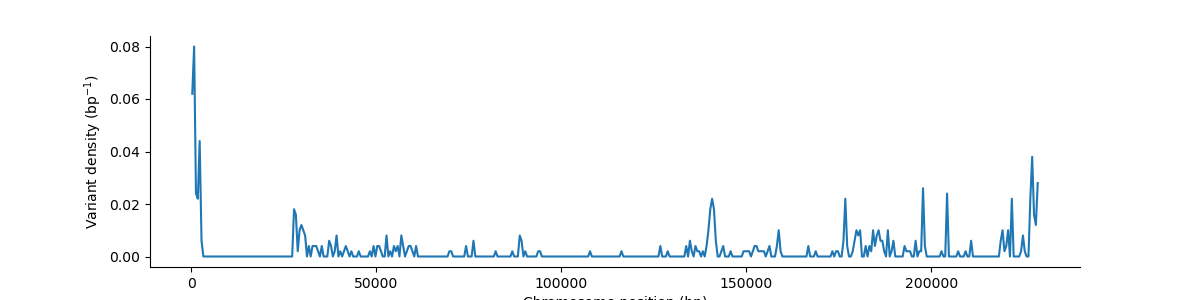
\includegraphics[width=.8\textwidth]{results/positions.png}
		
	\end{enumerate}
\end{frame}

%%%%%%%%%%%%%%%%%%%%%%%%%%%%%%%%%%%%%%%%%%%%%%%%%%%%%%%%%%%%%%%%%%%%%%%%%%%%%%%%
\subsection{Snakemake and external Scripts}

%%%%%%%%%%%%%%%%%%%%%%%%%%%%%%%%%%%%%%%%%%%%%%%%%%%%%%%%%%%%%%%%%%%%%%%%%%%%%%%%
\begin{frame}[fragile]
  \frametitle{\Snakemake{} Specials for Python}
  Sometime we have to start programs like this in \Snakemake:
  \begin{lstlisting}[language=Python,style=Python]
shell:  'some_command -i {input} -o {output}'
  \end{lstlisting}
  \begin{question}
  	If this would be a Python script $\ldots$ Isn't this rather tedious, considering that \Snakemake{} is written in Python? Could we forward rule specific information to our scripts?
  \end{question}
  \pause
  \begin{docs}
  	Remember: Not only are Snakefiles Python files, as our example with the \altverb{run} directive demonstrates: They inherit the same environment and namespace as our Snakefile. So, we must be able to use every information of the Snakefile within a script!
  \end{docs}
\end{frame}

\begingroup
\setbeamertemplate{footline}{}
%%%%%%%%%%%%%%%%%%%%%%%%%%%%%%%%%%%%%%%%%%%%%%%%%%%%%%%%%%%%%%%%%%%%%%%%%%%%%%%%
\begin{frame}[fragile]
  \frametitle{\Snakemake's features for external Scripts}
  In addition to the \altverb{shell} and \altverb{run} directives, \Snakemake{} offers a \altverb{script} directive, too:
  \begin{lstlisting}[language=Python,style=Python]
rule NAME:
    input:
        "path/to/inputfile",
    output:
        "path/to/outputfile",
    script:
        "scripts/script.py"
  \end{lstlisting}
  This lets you use (in \altverb{script.py}):
  \begin{lstlisting}[language=Python,style=Python]
def do_something(data_path, out_path):
    # python code

do_something(snakemake.input[0], snakemake.output[0])
  \end{lstlisting}
\end{frame}
\endgroup

%%%%%%%%%%%%%%%%%%%%%%%%%%%%%%%%%%%%%%%%%%%%%%%%%%%%%%%%%%%%%%%%%%%%%%%%%%%%%%%%
\begin{frame}[fragile]
  \frametitle{\Interlude{The same feature is offered for R}}
  \begin{lstlisting}[language=R,style=R]
do_something <- function(data_path, output_path) {
    # R code
}

do_something(snakemake@input[[1]], snakemake@output[[1]])
  \end{lstlisting}
\end{frame}

%%%%%%%%%%%%%%%%%%%%%%%%%%%%%%%%%%%%%%%%%%%%%%%%%%%%%%%%%%%%%%%%%%%%%%%%%%%%%%%%
\begin{frame}[fragile]
	\frametitle{\HandsOn{Write a Plotting Rule using the \texttt{script} Directive}}
	If you do not have a working workflow, refer to the solution \altverb{<++course.pathtosolutions++>/06_Snakefile_run}.\newline
	To prepare copy a plotting script into the \altverb{scripts} folder:
	\begin{lstlisting}[language=Bash, style=Shell, basicstyle=\footnotesize]
cp <++course.pathtosolutions++>\
/scripts/plot-quals.py scripts/.
    \end{lstlisting}
    Now, write a rule, which
    \begin{enumerate}
    	\item takes the vcf file as input
    	\item a plot file as output (same directory as for the first plot)
    	\item uses the \altverb{script}-directive and point to the script we just copied to our \altverb{scripts} directory.
    \end{enumerate}
\end{frame}

%%%%%%%%%%%%%%%%%%%%%%%%%%%%%%%%%%%%%%%%%%%%%%%%%%%%%%%%%%%%%%%%%%%%%%%%%%%%%%%%
\begin{frame}[fragile]
  \frametitle{Solution, plotting the Quality Scores}
  You will find the solution at \altverb{<++course.pathtosolutions++>/07_Snakefile_script}, too.
  \begin{lstlisting}[language=Python,style=Python]
rule plot_quals:
    input:
        "calls/all.vcf"
    output:
        "plots/quals.svg"
    @script:@
        "scripts/plot-quals.py"
  \end{lstlisting}
  \begin{hint}
  	You may choose any format offered by your matplotlib installation, it does not have to be \altverb{svg}.
  \end{hint}
  \pause
  \begin{question}
  	What is missing to start produce the desired plot?
  \end{question}
\end{frame}

%%%%%%%%%%%%%%%%%%%%%%%%%%%%%%%%%%%%%%%%%%%%%%%%%%%%%%%%%%%%%%%%%%%%%%%%%%%%%%%%
\begin{frame}[fragile]
	\frametitle{Solution: One more Target}
	
	Solution:
	\begin{lstlisting}[language=Python,style=Python]
rule all:
    input:
        "calls/all.vcf", # note the comma!
        "calls/positions.png",
        @"calls/quals.svg"@
	\end{lstlisting}
\end{frame}

\setcounter{preframe_handson}{\value{handson}}
%%%%%%%%%%%%%%%%%%%%%%%%%%%%%%%%%%%%%%%%%%%%%%%%%%%%%%%%%%%%%%%%%%%%%%%%%%%%%%%%
\begin{frame}[fragile]
  \frametitle{Disecting the Plotting Script}
  \setcounter{handson}{\value{preframe_handson}}

  \begin{onlyenv}<1| handout:0>
   We start with importing a plotting library
   \begin{lstlisting}[language=Python,style=Python]
@import matplotlib@
   \end{lstlisting}
  \end{onlyenv}
  \begin{onlyenv}<2| handout:0>
   We enforce writing to suppress the interactive mode:
   \begin{lstlisting}[language=Python,style=Python]
import matplotlib
@matplotlib.use("Agg")@
   \end{lstlisting}
  \end{onlyenv}
  \begin{onlyenv}<3| handout:0>
   We want an alternative interface:
   \begin{lstlisting}[language=Python,style=Python]
import matplotlib
matplotlib.use("Agg")
@import matplotlib.pyplot as plt@
   \end{lstlisting}
  \end{onlyenv}
  \begin{onlyenv}<4| handout:0>
   \ldots and need to import a function to read our variant file:
   \begin{lstlisting}[language=Python,style=Python]
import matplotlib
matplotlib.use("Agg")
import matplotlib.pyplot as plt
@from pysam import VariantFile@
   \end{lstlisting}
  \end{onlyenv}
  \begin{onlyenv}<5| handout:0>
   Let's start a list comprehension \ldots
   \begin{lstlisting}[language=Python,style=Python]
import matplotlib
matplotlib.use("Agg")
import matplotlib.pyplot as plt
from pysam import VariantFile

@quals = [@
   \end{lstlisting}
  \end{onlyenv}
   \begin{onlyenv}<6| handout:0>
   \ldots to construct a list of quality scores from our previous outputs:
   \begin{lstlisting}[language=Python,style=Python]
import matplotlib
matplotlib.use("Agg")
import matplotlib.pyplot as plt
from pysam import VariantFile

@quals = [record.qual for record 
         in VariantFile(snakemake.input[0])]@
   \end{lstlisting}
  \end{onlyenv}
  \begin{onlyenv}<7| handout:0>
   Finally, plot a histogram \ldots
   \begin{lstlisting}[language=Python,style=Python]
import matplotlib
matplotlib.use("Agg")
import matplotlib.pyplot as plt
from pysam import VariantFile

quals = [record.qual for record 
         in VariantFile(snakemake.input[0])]
         
@plt.hist(quals)@
   \end{lstlisting}
  \end{onlyenv}
  \begin{onlyenv}<8| handout:0>
   \ldots and save the figure.
   \begin{lstlisting}[language=Python,style=Python]
import matplotlib
matplotlib.use("Agg")
import matplotlib.pyplot as plt
from pysam import VariantFile

quals = [record.qual for record 
         in VariantFile(snakemake.input[0])]
         
plt.hist(quals)
@plt.savefig(snakemake.output[0])@
   \end{lstlisting}
  \end{onlyenv}
  \begin{onlyenv}<9| handout:1>
   This should be our final script:
   \begin{lstlisting}[language=Python,style=Python]
import matplotlib
matplotlib.use("Agg")
import matplotlib.pyplot as plt
from pysam import VariantFile

quals = [record.qual for record 
         in VariantFile(snakemake.input[0])]
         
plt.hist(quals)
plt.savefig(snakemake.output[0])
   \end{lstlisting}
  To be copied from \altverb{<++course.pathtosolutions++>/07_Snakefile_script} to \altverb{scripts/plot-quals.py} - if you have not done so, already.
  \end{onlyenv}
\end{frame}

%%%%%%%%%%%%%%%%%%%%%%%%%%%%%%%%%%%%%%%%%%%%%%%%%%%%%%%%%%%%%%%%%%%%%%%%%%%%%%%%
\begin{frame}[fragile]
	\frametitle{\Interlude{Debugging external Scripts}}
	\begin{exampleblock}{Debugging Python Scripts}
		To debug Python scripts, you can invoke \Snakemake{} with
		\begin{lstlisting}[language=Bash, style=Shell]
$ snakemake --debug
		\end{lstlisting}
		As always in Python, you may use \altverb{print()} and \altverb{logging()} functions which may write to a log file during the run to check whether the script behaves as expected.
	\end{exampleblock}
	\pause
	\begin{exampleblock}{Debugging R Scripts}
		To debug R scripts, you can save the workspace with \altverb{save.image()}, and invoke R after \Snakemake{} has terminated. 
	\end{exampleblock}
\end{frame}

%%%%%%%%%%%%%%%%%%%%%%%%%%%%%%%%%%%%%%%%%%%%%%%%%%%%%%%%%%%%%%%%%%%%%%%%%%%%%%%%
\subsection{Running the final Workflow}

%%%%%%%%%%%%%%%%%%%%%%%%%%%%%%%%%%%%%%%%%%%%%%%%%%%%%%%%%%%%%%%%%%%%%%%%%%%%%%%%
\begin{frame}[fragile]
	\frametitle{\HandsOn{Executing this Workflow}}
	\begin{task}
		Does our Workflow contain errors? We run a debug trial:
		\begin{lstlisting}[language=Bash, style=Shell]
$ snakemake --debug
		\end{lstlisting}
	\end{task}
	\pause
	Some targets are already present, we want the entire workflow again:
	\begin{lstlisting}[language=Bash, style=Shell]
$ snakemake -c4 --forcerun
$ # or short with
$ snakemake -c4 -F
	\end{lstlisting}
     
	\begin{question}
		What do you observe? Why \altverb{-c4}?
	\end{question}
\end{frame}

%%%%%%%%%%%%%%%%%%%%%%%%%%%%%%%%%%%%%%%%%%%%%%%%%%%%%%%%%%%%%%%%%%%%%%%%%%%%%%%%
\begin{frame}[fragile]
	\frametitle{\HandsOn{Visualising the Output}}
	On <++cluster.name++> the Linux distro is "<++cluster.distro++>", which \newline provides the \altverb{<++cluster.display_program++>}-program to display simple images. We shall invoke:
	\begin{lstlisting}[language=Bash, style=Shell]
$ <++cluster.display_program++> calls/quals.svg
	\end{lstlisting}
	The figure has no axis-labels.
	\begin{question}
		What does the figure display?
	\end{question}
\end{frame}

%%%%%%%%%%%%%%%%%%%%%%%%%%%%%%%%%%%%%%%%%%%%%%%%%%%%%%%%%%%%%%%%%%%%%%%%%%%%%%%%
\begin{frame}[fragile]
	\frametitle{\HandsOn{Moving \altverb{run} to \altverb{script}}}
	\footnotesize
	\begin{question}
		Take a look at the \altverb{plot_positions} rule, once more: Is it a good idea to have this much code inlined in a Snakefile? When is it a good idea?
	\end{question}
	\pause
	\begin{docs}
		Only place a few lines in a \altverb{run} directive, i.\,e. to copy files or to trigger a download from within Python.
	\end{docs}
	\pause
	\begin{task}
		Copy the content of \altverb{plot_positions} into a script file. Save it as a Python script (suffix: \altverb{.py}) in the \altverb{scripts} folder. You need to change the \altverb{run} directive.\newline
		\textbf{Attention:} Start the script with 0 indentation; preserve the relative indentation.\newline
		\textbf{Remember:} Within a script \altverb{input} and \altverb{output} are accessible in the \altverb{snakemake} object, compare to the \altverb{plot-quals.py} script.
	\end{task}
\end{frame}

%%%%%%%%%%%%%%%%%%%%%%%%%%%%%%%%%%%%%%%%%%%%%%%%%%%%%%%%%%%%%%%%%%%%%%%%%%%%%%%%
\begin{frame}[fragile]
	\frametitle{Solution}
	\begin{lstlisting}[language=Python,style=Python]
rule plot_quals:
    input:
        "calls/all.vcf"
    output:
        "call/positions.png"
    @script:@
        "scripts/plot-positions.py"
	\end{lstlisting}
	Compare to the solution script in your solutions folder: \altverb{<++course.pathtosolutions++>/08_Snakefile_script2}.
\end{frame}

%%%%%%%%%%%%%%%%%%%%%%%%%%%%%%%%%%%%%%%%%%%%%%%%%%%%%%%%%%%%%%%%%%%%%%%%%%%%%%%%
\begin{frame}<handout:0>
	\frametitle{Our ``final'' Workflow}
	Let us check our -- so far -- final workflow, together.
\end{frame}







